\documentclass[usenames,dvipsnames,tikz]{standalone}
%\usepackage{amsmath,amssymb}
%\usepackage{xcolor}
\colorlet{tBlue}{RoyalBlue!35!Cerulean}
\colorlet{tRed}{Red}
%\usepackage{tikz}
%\usepackage{standalone}
\begin{document}
	
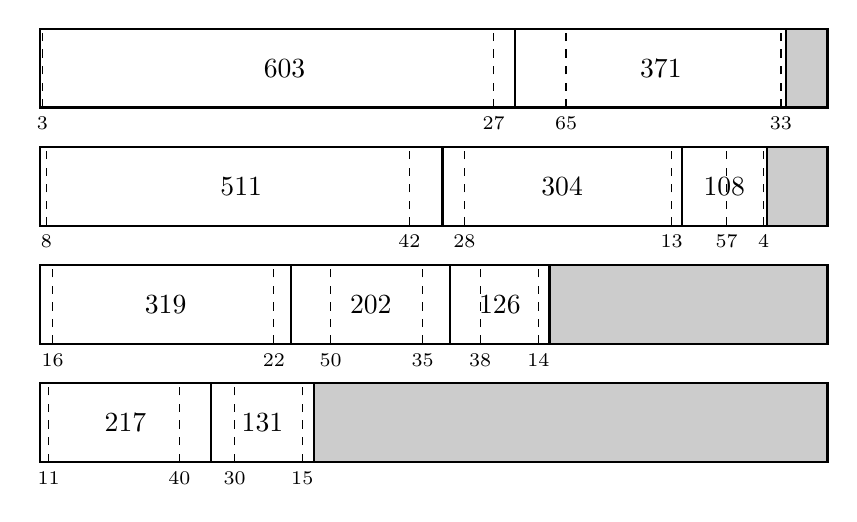
\begin{tikzpicture}
%\draw [help lines] (-1,-2) grid (12,5);
% 1=0.1, 2=0.15, 3=0.2, 4=0.25, 5=0.3
% 6 (3-27), 5 (8-42), 4 (33-65), 4 (16-22), 3 (13-28), 3 (11-40), 2 (35-50), 1 (15-30), 1 (14-38), 1 (4-57).

\draw [thick] (0,0) rectangle (10,1);
\draw [thick] (0,1.5) rectangle (10,2.5);
\draw [thick] (0,3) rectangle (10,4);
\draw [thick] (0,4.5) rectangle (10,5.5);

% Bottom row, 217, 131 (11-40, 30-15, sixth, tenth)
\draw [thick] (2.17,0) -- (2.17,1);
\draw [thick] (3.48,0) -- (3.48,1);
\filldraw[fill=black!20!white, draw=black, thick] (3.48,0) rectangle (10,1);

\draw [dashed] (0.11,0) -- (0.11,1);
\draw [dashed] (1.77,0) -- (1.77,1);
\node [below] at (0.11,0) {\scriptsize{$11$}};
\node [below] at (1.77,0) {\scriptsize{$40$}};

\draw [dashed] (2.47,0) -- (2.47,1);
\draw [dashed] (3.33,0) -- (3.33,1);
\node [below] at (2.47,0) {\scriptsize{$30$}};
\node [below] at (3.33,0) {\scriptsize{$15$}};

\node at (1.085,0.5) {217};
\node at (2.825,0.5) {131};

% Second from bottom row, 319, 202, 126 (16-22, 50-35, 38-14, fourth, seventh, ninth)
\draw [thick] (3.19,1.5) -- (3.19,2.5);
\draw [thick] (5.21,1.5) -- (5.21,2.5);
\draw [thick] (6.47,1.5) -- (6.47,2.5);
\filldraw[fill=black!20!white, draw=black, thick] (6.47,1.5) rectangle (10,2.5);

\draw [dashed] (0.16,1.5) -- (0.16,2.5);
\draw [dashed] (2.97,1.5) -- (2.97,2.5);
\node [below] at (0.16,1.5) {\scriptsize{$16$}};
\node [below] at (2.97,1.5) {\scriptsize{$22$}};

\draw [dashed] (3.69,1.5) -- (3.69,2.5);
\draw [dashed] (4.86,1.5) -- (4.86,2.5);
\node [below] at (3.69,1.5) {\scriptsize{$50$}};
\node [below] at (4.86,1.5) {\scriptsize{$35$}};

\draw [dashed] (5.59,1.5) -- (5.59,2.5);
\draw [dashed] (6.33,1.5) -- (6.33,2.5);
\node [below] at (5.59,1.5) {\scriptsize{$38$}};
\node [below] at (6.33,1.5) {\scriptsize{$14$}};

\node at (1.595,2) {$319$};
\node at (4.2,2) {$202$};
\node at (5.84,2) {$126$};

% Second from top row, 511, 304, 108 (8-42, 28-13, 57-4, second, fifth, eighth)
\draw [thick] (5.11,3) -- (5.11,4);
\draw [thick] (8.15,3) -- (8.15,4);
\draw [thick] (9.23,3) -- (9.23,4);
\filldraw[fill=black!20!white, draw=black, thick] (9.23,3) rectangle (10,4);

\draw [dashed] (0.08,3) -- (0.08,4);
\draw [dashed] (4.69,3) -- (4.69,4);
\node [below] at (0.08,3) {\scriptsize{$8$}};
\node [below] at (4.69,3) {\scriptsize{$42$}};

\draw [dashed] (5.39,3) -- (5.39,4);
\draw [dashed] (8.02,3) -- (8.02,4);
\node [below] at (5.39,3) {\scriptsize{$28$}};
\node [below] at (8.02,3) {\scriptsize{$13$}};

\draw [dashed] (8.72,3) -- (8.72,4);
\draw [dashed] (9.19,3) -- (9.19,4);
\node [below] at (8.72,3) {\scriptsize{$57$}};
\node [below] at (9.19,3) {\scriptsize{$4$}};

\node at (2.555,3.5) {$511$};
\node at (6.63,3.5) {$304$};
\node at (8.69,3.5) {$108$};

% Top row, 603, 371 (3-27, 65-33, first, third)
\draw [thick] (6.03,4.5) -- (6.03,5.5);
\filldraw[fill=black!20!white, draw=black, thick] (9.47,4.5) rectangle (10,5.5);

\draw [dashed] (0.03,4.5) -- (0.03,5.5);
\draw [dashed] (5.76,4.5) -- (5.76,5.5);
\node [below] at (0.03,4.5) {\scriptsize{$3$}};
\node [below] at (5.76,4.5) {\scriptsize{$27$}};

\draw [dashed] (6.68,4.5) -- (6.68,5.5);
\draw [dashed] (9.41,4.5) -- (9.41,5.5);
\node [below] at (6.68,4.5) {\scriptsize{$65$}};
\node [below] at (9.41,4.5) {\scriptsize{$33$}};

\node at (3.105,5) {$603$};
\node at (7.885,5) {$371$};


\end{tikzpicture}

\end{document}